\documentclass[a4paper]{article}
\usepackage[T1]{fontenc}
\usepackage[utf8]{inputenc}
\usepackage[italian]{babel}
\usepackage{booktabs}
\usepackage{graphicx}
\usepackage{hyperref}
\usepackage{verbatim}
\usepackage{geometry}
\usepackage{textcomp}
\usepackage{listings}
\geometry{a4paper,top=2cm,bottom=2.5cm,left=2.5cm,right=2.5cm}
\usepackage{xcolor}
\lstset{
  language=bash,
  backgroundcolor=\color{black},
  basicstyle=\scriptsize\color{white}\ttfamily\bfseries,
  keywordstyle=\color{blue},
  showstringspaces=false,
  columns=fullflexible
}


\begin{document}


\author{Leo Paolo}
\title{Manuale codice Picoscope}
\maketitle

\section{Settare ambiente e librerie Picoscope}
Questo capitolo è una guida ad installare il software e impostare l'ambiente di lavoro per poter utilizzare il codice d'esempio reso disponibile dagli sviluppatori Picoscope per c/c++. Parte di ciò che verrà detto in questo capitolo è presente all'indirizzo \url{https://github.com/picotech/picosdk-c-examples}, insieme al codice d'esempio che utilizzeremo. Se l'ambiente di lavoro è già impostato andate al capitolo successivo. \\
\\
\\
\noindent Presupponendo di avere una macchina Linux, aprire il terminale ed eseguire i seguenti comnadi:
\begin{lstlisting}[language=bash]
sudo apt-get install libps5000a
\end{lstlisting}
Questo comando installerà le librerie necessarie per poter utilizzare il codice d'esempio del Picoscope.\\
\noindent Adesso, andate nella cartella:
\begin{lstlisting}[language=bash]
cd /opt/picoscope/share/doc/libps5000a
\end{lstlisting}
Collegate il Picoscope attraverso la porta USB al vostro computer ed eseguite il comando:
\begin{lstlisting}[language=bash]
./usbtest
\end{lstlisting}
Se il Picoscope è alimentato, collegato al vostro pc, e avete installato con successo la libreria necessaria, dovreste ottenere un output simile a questo:
\begin{figure}[h!]
\centering
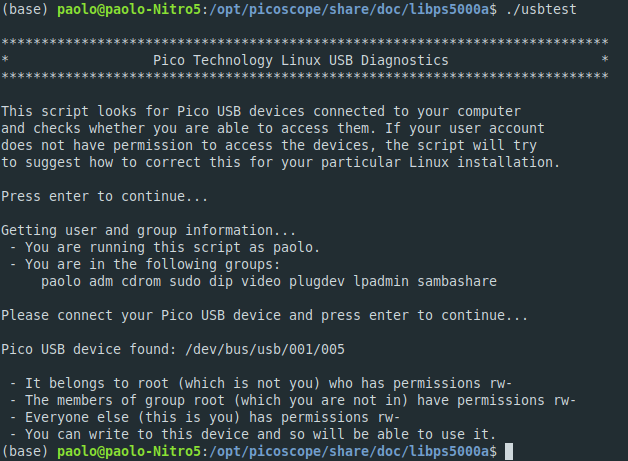
\includegraphics[scale=0.26]{Immagini/usbtest.png}
\end{figure}
Adesso che ci siamo assicurati che la libreria è installata correttamente, scarichiamo in una cartella apposita tutti i file d'esempio disponibili all'indirizzo github:
\begin{lstlisting}[language=bash]
git clone https://github.com/picotech/picosdk-c-examples
\end{lstlisting}
Una volta scaricato, andate nella cartella:
\begin{lstlisting}[language=bash]
cd ps5000a/linux-build-files/
\end{lstlisting}
Dove "ps5000a" è la libreria che utilizzeremo per la nostra versione del Picoscope (5444D). Una volta in questa cartella copiate il file che si trova nella cartella "ps5000aCon":
\begin{lstlisting}[language=bash]
cp ../ps5000aCon/ps5000aCon.c .
\end{lstlisting}
e usate il seguente comando:
\begin{lstlisting}[language=bash]
./autogen.sh
\end{lstlisting}
Adesso è possibile incorrere in una serie di errori, di cui elenco le soluzioni:
\begin{enumerate}
\item \begin{lstlisting}[language=bash]
Can't exec "aclocal": No such file or directory at /usr/share/autoconf/Autom4te/FileUtils.pm line 326.
autoreconf: failed to run aclocal: No such file or directory
\end{lstlisting}
Soluzione:
\begin{lstlisting}[language=bash]
sudo apt-get install automake
\end{lstlisting}

\item \begin{lstlisting}[language=bash]
configure: error: libps5000a-1.1/ps5000aApi.h missing!
\end{lstlisting}
Soluzione:
Bisogna rimuovere dai seguenti file presenti nella attuale cartella: \verb|configure.ac| e \verb|ps5000aCon.c| tutti i riferimenti alle librerie \verb|libps5000a-1.1| in questo modo:\\
\verb|libps5000a-1.1|$\to$\verb|libps5000a| oppure \verb|...-1.1|$\to$\verb|...|
\end{enumerate}
Una volta risolti gli eventuali errori eseguire il seguente comando:
\begin{lstlisting}[language=bash]
make
\end{lstlisting}
Se appare questo output sul terminale:
\begin{lstlisting}[language=bash]
make  all-am
make[1]: Entering directory '/home/md13/Desktop/Fermilab/Magnetometer/INO/picosdk_C/ps5000a/linux-build-files'
CC       ps5000aCon.o
CCLD     ps5000aCon
make[1]: Leaving directory '/home/md13/Desktop/Fermilab/Magnetometer/INO/picosdk_C/ps5000a/linux-build-files'
\end{lstlisting}
Allora tutto ok! Dovrebbe essere presente adesso nella cartella un eseguibile che è possibile lanciare con il comando:
\begin{lstlisting}[language=bash]
./ps5000aCon
\end{lstlisting}


\section{Utilizzare il codice}
\end{document}
